\documentclass[11pt,a4paper]{article}
\usepackage[utf8]{inputenc}
\usepackage[spanish]{babel}
\usepackage{amsmath}
\usepackage{amsfonts}
\usepackage{amssymb}
\usepackage{graphicx}
\usepackage[left=2cm,right=2cm,top=2cm,bottom=2cm]{geometry}
\usepackage{listings}
\usepackage[hidelinks]{hyperref}
\usepackage{lscape}
\usepackage{rotating}
\usepackage{pdflscape}

\lstset{
basicstyle=\ttfamily,
frame=single,
language=SQL,
tabsize=2,
showstringspaces=false,
literate=%
    {á}{{\'a}}1
    {é}{{\'e}}1
    {è}{{\`e}}1
    {í}{{\'i}}1
    {ó}{{\'o}}1
    {ú}{{\'u}}1
}

\begin{document}

\begin{titlepage}
	\title{{\Huge \textbf{Práctica 4 - Bases de Datos 2}}}
	\author{
	  Hayk Kocharyan\\
	  757715@unizar.es
	  \and
	  Juan José Tambo Tambo\\
	  755742@unizar.es
	  \and
	  Pedro Tamargo Allué\\
	  758267@unizar.es
	  \and
	  Jesús Villacampa Sagaste\\
	  755739@unizar.es
	}
	\date{\today}
	
	\clearpage\maketitle
	\thispagestyle{empty}
	\tableofcontents
	\listoffigures
\end{titlepage}

\section{Esfuerzos invertidos}

\begin{itemize}
\item Hayk:
\item Juan José:
\item Pedro:
\item Jesús:
\end{itemize}

\section{Modelo conceptual}

Durante el desarrollo de la práctica 1 se diseñó una base de datos para un banco que quería gestionar cuentas con múltiples propietarios, diferentes tipos de cuentas (cuentas ahorro y cuentas corrientes), operaciones (transacciones entre cuentas, o movimientos de dinero en efectivo) y las sucursales de la entidad.\\
En la Figura \ref{fig:diagramaer} se puede observar el esquema entidad relación sobre el problema planteado. Se ha planteado las relaciones entre los distintos tipos de cuentas como una generalización, ya que todas comparten ciertos atributos como el número de cuenta, el \emph{IBAN}, la fecha de apertura y el saldo restante. Esta generalización es exclusiva ya que no se considera posible la capacidad de que una cuenta pertenezca a los dos tipos de entidades al mismo tiempo. También, se trata de una generalización total ya que no se considera el caso de que una cuenta no pertenezca a algunos de las entidades derivadas de \emph{Cuenta}.\\
Con transacción ocurre lo mismo, una transferencia entre cuentas y las operaciones de retirada o ingreso de efectivo se pueden generalizar en una nueva entidad \emph{Transacción} con los atributos comunes a ambas entidades, tales como: el número de la transacción, la fecha y hora de la misma, su importe y una descripción a modo de concepto. Se trata de una generalización exclusiva ya que una transferencia no puede pertenecer a los dos subtipos a la vez. También, se trata de una generalización total ya que en el contexto del problema no tiene sentido que exista una transferencia que no pertenezca a \emph{Operación (operaciones en efectivo)} o a \emph{Transferencia (transferencia de saldo entre cuentas)}.\\
Se ha decidido que \emph{Transacción} debía ser débil respecto a \emph{cuenta} ya que depende en existencia e identificación de \emph{cuenta}, por lo tanto la relación \emph{Realizar} es una relación \emph{1:N} entre \emph{Cuenta} y \emph{Transacción}. No obstante, existe una transacción que no indica la debilidad de la entidad \emph{Transacción} respecto a \emph{Cuenta}, la relación \emph{Recibir}, una relación \emph{1:N} que relaciona las entidades \emph{Cuenta} y \emph{Transferencia} , y cuyo significado es relacionar una transferencia con la cuenta beneficiaria.\\
Los clientes titulares de una cuenta se reflejan en la entidad \emph{Cliente}, que almacena el DNI, el nombre, los apellidos la dirección y el email. Se ha decidido que el \emph{DNI} sea la clave primaria ya que es único para los ciudadanos.\\
La relación de \emph{Cliente} con \emph{Cuenta} se encuentra en \emph{Poseer}, una relación \emph{M:N} que posibilita que una cuenta tenga más de un titular.\\
Para el almacenamiento de las sucursales de la entidad bancaria, se ha diseñado una entidad \emph{Sucursal}, que almacena el código de la entidad, su dirección postal y el teléfono de la oficina. Se ha decidido que el código de la sucursal sea la clave primaria que identifique a las sucursales ya que dentro de la misma entidad bancaria no existen dos sucursales con el mismo código.\\
Se ha considerado que las transacciones se tienen que realizar en una sucursal, por lo tanto existe una relación entre \emph{Transacción} y \emph{Sucursal}. También, una cuenta corriente debe ser abierta en una determinada sucursal de la entidad.\\

Como apoyo hacia el desarrollo orientado a objetos con \emph{Java} se ha utilizado como referencia un diagrama de clases \emph{UML} (Figura \ref{fig:diagramauml}) con la misma semántica que el diagrama entidad relación explicado anteriormente.\\

\textbf{Aquí explicaremos el diagrama ER de banquito, para que lo tengan presente (Figura \ref{fig:diagramaer}).}

\section{Entorno de trabajo y ejecución}

Para la realización de la práctica se ha utilizado la herramienta \emph{Apache Maven\footnote{\url{https://maven.apache.org/}}} para compilar, gestionar las dependencias y ejecutar el código.\\
Como entorno de desarrollo se va a utilizar \emph{Visual Studio Code\footnote{\url{https://code.visualstudio.com/}}}, un editor de código abierto que tiene integraciones con diferentes herramientas (como \emph{Maven}) y lenguajes de programación.\\

Para configurar la herramienta \emph{Maven} debemos crear un proyecto con la forma especificada en la Figura \ref{fig:estructuraMAVEN}. El fichero \emph{pom.xml} (\emph{Project Object Model}) se corresponde con el fichero que utiliza \emph{Maven} para gestionar las dependencias y establecer distintas etapas del ciclo de vida del código, tales como \emph{COMPILE}, \emph{EXEC} o \emph{CLEAN}.\\
Para no utilizar un fichero \emph{pom.xml} vacío desde 0, se ha procedido a utilizar un \emph{archetype}, el cual proporciona una estructura básica. El \emph{archetype} utilizado ha sido: \emph{archetype-quickstart-jdk8}.\\
El código se desarrollará en el directorio \emph{src/main/java/package-name}, donde \emph{package-name} se corresponde con el \emph{groupId} especificado en el fichero \emph{pom.xml}.\\
Para ejecutar el código generado primero debemos compilarlo, para ello, desde la línea de comandos del sistema operativo, en el mismo directorio donde se encuentre el fichero \emph{pom.xml} escribiremos la siguiente orden:

\begin{lstlisting}
# Limpiamos los resultados de una ejecución anterior
mvn clean
# Primero compilamos el código Java
mvn compile
# Donde package-name se corresponde con el groupId especificado.
mvn exec:java -Dexec.mainClass="package-name.App"
\end{lstlisting}

Para añadir las dependencias de los distintos \emph{JAR} que necesite el proyecto, hay que añadirlas en el apartado \emph{dependencies} del fichero \emph{pom.xml} de la siguiente forma:

\begin{lstlisting}
<dependencies>
	<dependency>
		<groupId>org.junit.jupiter</groupId>
		<artifactId>junit-jupiter-api</artifactId>
		<version>${junit.version}</version>
		<scope>test</scope>
	</dependency>
	<dependency>
		<groupId>org.junit.jupiter</groupId>
		<artifactId>junit-jupiter-engine</artifactId>
		<version>${junit.version}</version>
		<scope>test</scope>
	</dependency>
	<!--  Driver JDBC Oracle  -->
	<dependency>
		<groupId>com.oracle.database.jdbc</groupId>
		<artifactId>ojdbc8</artifactId>
		<version>19.6.0.0</version>
	</dependency>
	<!--  Jar de Hibernate Core  -->
	<dependency>
		<groupId>org.hibernate</groupId>
		<artifactId>hibernate-core</artifactId>
		<version>5.4.15.Final</version>
	</dependency>
	<!--  Jar de entity manager  -->
	<dependency>
		<groupId>org.hibernate</groupId>
		<artifactId>hibernate-entitymanager</artifactId>
		<version>5.4.15.Final</version>
	</dependency>
	<!--  javax.persistence  -->
	<dependency>
		<groupId>javax.persistence</groupId>
		<artifactId>persistence-api</artifactId>
		<version>1.0.2</version>
	</dependency>
</dependencies>
\end{lstlisting}

Siendo cada elemento entre las etiquetas \emph{dependency} una dependencia que \emph{Maven} tiene que resolver. Para obtener la información acerca de la dependencia se puede consultar el repositorio de \emph{Maven Central\footnote{\url{https://search.maven.org/}}}. En este repositorio se puede realizar una búsqueda de la dependencia y obtener información de la misma. En la Figura \ref{fig:mavenCentral} se puede observar el resultado de la búsqueda del driver \emph{JDBC} de \emph{Oracle} utilizando este sistema. En la parte derecha de la misma se puede observar que se proporciona la etiqueta \emph{dependency} que ha sido añadida al fichero \emph{pom.xml}.\\

Tras la configuración de la herramienta es necesaria la configuración de \emph{JPA}, a partir del fichero \emph{persistence.xml}. Este fichero debe esta alojado en el \emph{Classpath} del proyecto, dentro del directorio \emph{META-INF}. Por lo tanto se ha creado un directorio \emph{src/main/resources/META-INF/} en el cual se alojará este fichero. Para la configuración de la unidad de persistencia se utilizará la base de datos \emph{Oracle} ubicada en \emph{danae04.cps.unizar.es}. El fichero \emph{persistence.xml} tendrá la siguiente forma:

\begin{lstlisting}
<persistence xmlns="http://java.sun.com/xml/ns/persistence"
             xmlns:xsi="http://www.w3.org/2001/XMLSchema-instance"
             xsi:schemaLocation="http://java.sun.com/xml/ns/persistence 
             http://java.sun.com/xml/ns/persistence/persistence_2_0.xsd" 
             version="2.0">
	<persistence-unit name="UnidadPersistenciaAlumnos"
			 transaction-type="RESOURCE_LOCAL">
		<provider>org.hibernate.ejb.HibernatePersistence</provider>
		<properties>
		   <property name="hibernate.dialect" 
		   	value="org.hibernate.dialect.Oracle8iDialect" />
		   <property name="hibernate.show_sql" value="true"/>		
		   <property name="hibernate.hbm2ddl.auto" value="create"/>
		  
		   
		   <property name="javax.persistence.jdbc.driver" 
		   	value="oracle.jdbc.driver.OracleDriver"/>
		   <property name="javax.persistence.jdbc.url" 
		   	value="jdbc:oracle:thin:@danae04.cps.unizar.es:1521:barret"/>
		   <property name="javax.persistence.jdbc.user" value=""/>
		   <property name="javax.persistence.jdbc.password" value=""/>		   
		   

		</properties>
	</persistence-unit>
</persistence>
\end{lstlisting}

Tras la ejecución del código \emph{JPA} puede aparecer este error:

\begin{lstlisting}
[WARNING] thread Thread[Timer-0,5,bases2.App] was interrupted but is 
	still alive after waiting at least 15000msecs
[WARNING] thread Thread[Timer-0,5,bases2.App] will linger despite 
	being asked to die via interruption
[WARNING] thread Thread[InterruptTimer,5,bases2.App] will linger 
	despite being asked to die via interruption
[WARNING] thread Thread[Hibernate Connection Pool Validation 
	Thread,5,bases2.App] will linger despite being asked to die 
	via interruption
[WARNING] NOTE: 3 thread(s) did not finish despite being asked to 
	via interruption. This is not a problem with exec:java, 
	it is a problem with the running code. 
	Although not serious, it should be remedied.
[WARNING] Couldn't destroy threadgroup 
	org.codehaus.mojo.exec.ExecJavaMojo$IsolatedThreadGroup
	[name=bases2.App,maxpri=10]
java.lang.IllegalThreadStateException
    at java.lang.ThreadGroup.destroy (ThreadGroup.java:776)
    at [...]
\end{lstlisting}

Este error es debido a que en el final del código un proceso \emph{Daemon} se encarga de monitorizar que todos los hilos (\emph{Threads}) terminen correctamente. Para solventar este error podemos utilizar este otro comando para ejecutar el código:

\begin{lstlisting}
mvn exec:java 
	-Dexec.mainClass="package-name.App" 
	-Dexec.cleanupDaemonThreads=false
\end{lstlisting}

\textbf{Aquí le explicaremos que usamos visual code con maven y le explicaremos como se ejecuta.}

\section{Generación de esquema lógico con JPA}

Para la generación del esquema lógico utilizando \emph{JPA} se ha  utilizado el diagrama de clases de la Figura \ref{fig:diagramauml}. El primer paso de la generación ha sido la confección de las clases \emph{Java} utilizando las anotaciones necesarias. En este caso, se han utilizado las anotaciones \emph{@Entity} para marcar las entidades y las etiquetas \emph{@Column} para las columnas. Para las columnas se ha añadido un atributo \emph{name} para especificar el nombre de esa columna en la base de datos y así conocer los nombres de las columnas.\\
Para que \emph{JPA} funcione correctamente se deben definir los métodos \emph{hashCode() y equals()}. También, en el ámbito de las consultas es conveniente definir un método \emph{toString()} para obtener una salida comprensible del contenido de cada uno de los objetos. También es necesario que las clases tengan una estructura tipo \emph{Java Bean\footnote{\url{https://es.wikipedia.org/wiki/JavaBean}}}, esto implica que las clases deben disponer de un constructor por defecto (se llama sin parámetros) y métodos \emph{getters} y \emph{setters} para el acceso directo a cada uno de sus atributos, que deberán ser marcados como privados para impedir su acceso directo desde fuera de la propia clase.\\
Para resolver la herencia en este primer esquema lógico se ha decidido establecer las \emph{superclases} \emph{Cuenta} y \emph{Transacción} como clases abstractas. De esta manera no podrán ser instanciadas y por lo tanto se obligará a que la herencia sea obligatoria. Además al utilizar dos subclases, la herencia será disjunta ya que un objeto no puede pertenecer a dos subclases al mismo tiempo en este modelo conceptual.\\
El mecanismo predeterminado para la resolución de estas herencias ha sido el de crear una sola tabla con el nombre del padre con todos los atributos del padre y los específicos de cada uno de los hijos. Para determinar si una tupla en la base de datos pertenece a un subtipo o a otro se dispone de una columna (por defecto, \emph{DTYPE}) que contiene el nombre del subtipo cuyos valores se encuentran con valores permitidos para ese subtipo.\\
Sobre las relaciones, se ha utilizado una relación \emph{ManyToMany} bidireccional entre \emph{Cliente} y \emph{Cuenta}, siendo cliente la parte poseedora. Esta acción genera una tabla nueva \emph{Cliente\_{}Cuenta}, que representará lo mismo que la tabla \emph{Poseer} de la base de datos de \emph{Banquito}.\\
No se han utilizado más relaciones bidireccionales pero es de destacar la relación \emph{ManyToOne} unidireccional entre \emph{Transacción} y \emph{Cuenta}, ya que transacción es una entidad débil ante cuenta. La columna resultante de esta relación actúa también como parte de la clave primaria al utilizarse la anotación \emph{@Id}, siendo la clave primaria \emph{(NumTransaccion, realizante)}.\\


\textbf{Aquí explicaremos como hemos desarrollado el esquema lógico desde 0 con JPA.}

\section{Adopción de un esquema lógico preexistente con JPA}

Partiendo de las clases desarrolladas en el apartado anterior, se va a proceder a realizar las modificaciones sobre las mismas para adaptar al esquema lógico existente. Esta tarea no ha resultado especialmente difícil ya que \emph{JPA} provee muchas anotaciones para modificar el comportamiento del esquema que se va a generar o que se va a adoptar. Para facilitar esta tarea se ha modificado un campo del fichero \emph{persistence.xml}, el campo \emph{hibernate.hbm2ddl.auto} adoptará el valor \emph{validate}. Esto comprobará si el esquema generado por \emph{JPA} coincide con el esquema existente en el remoto especificado en ese mismo fichero. No realiza ninguna modificación sobre la base de datos.\\
Para dejar claro el nombre de las tablas sobre las que actúan cada una de las entidades (\emph{@Entity}) desarrolladas se va a utilizar la anotación (\emph{@Table(name = "[...]")}) .\\
Las relaciones desarrolladas anteriormente se han mantenido, no obstante se ha utilizado la anotación \emph{@JoinColumn} para establecer atributos tales como el nombre de la columna, restricciones de unicidad.\\
En la relación \emph{ManyToMany} entre \emph{Cliente} y \emph{Cuenta} se ha utilizado la anotación \emph{@JoinTable} de la siguiente manera:

\begin{lstlisting}
@ManyToMany(fetch = FetchType.LAZY, cascade = CascadeType.ALL)
@JoinTable(
  name = "POSEER",
  joinColumns = @JoinColumn(
    referencedColumnName = "DNI",	name = "DNI"
  ),
  inverseJoinColumns = @JoinColumn(
    referencedColumnName = "NUM_CUENTA", name = "NUM_CUENTA"
  )
)
private List<Cuenta> cuentas;
\end{lstlisting}

Con esta anotación se ha establecido que la relación entre cliente y cuenta se establecerá sobre una tabla \emph{POSEER} con columnas \emph{DNI} referenciando a \emph{Cliente.DNI} y con la columna \emph{NUM\_{}CUENTA} referenciando a \emph{Cuenta.NUM\_{}CUENTA}.\\

Sobre la herencia, se han utilizado distintas estrategias de las propuestas por \emph{JPA}, en este caso, para la tabla cuenta se ha utilizado la estrategia \emph{JOINED}, la cual divide los campos específicos de la tabla padre en una tabla y los campos específicos de cada subtipo en sus respectivas tablas. En las tablas de los subtipos para establecer el nombre de la columna que actúa como clave primaria se utiliza la anotación \emph{@PrimaryKeyJoinColumn} con el atributo \emph{name}, en este caso se establecerá \emph{name = ``ID\_{}CUENTA''} para que coincidan con el esquema lógico preexistente.\\
En el caso de la herencia entre \emph{Transacción, Transferencia y Operación}, se ha establecido un mecanismo de herencia distinto. En este caso la superclase (transacción) no será una entidad, si no que se utilizará la anotación \emph{@MappedSuperclass} para indicar que esta superclase no se persistirá como una tabla en la base de datos, pero sus campos si que serán persistidos en cada uno de sus subtipos (transferencia y operación).

\textbf{Aquí le explicaremos el proceso de acomodación del esquema relacional de la base de datos con JPA. Le explicaremos lo del \emph{validate} y le mostraremos nuestros problemas.}

\section{Consultas con JPA}

\textbf{Aquí se expondrán las consultas, con su código SQL, JPQL, Criteria API}.

\section{Conclusiones y opiniones}

\textbf{Meter aqui las conclusiones y opiniones del equipo ante el uso de este ORM.}

\newpage
\section{Apéndice 1: Figuras}

\begin{landscape}
\begin{figure}
\centering
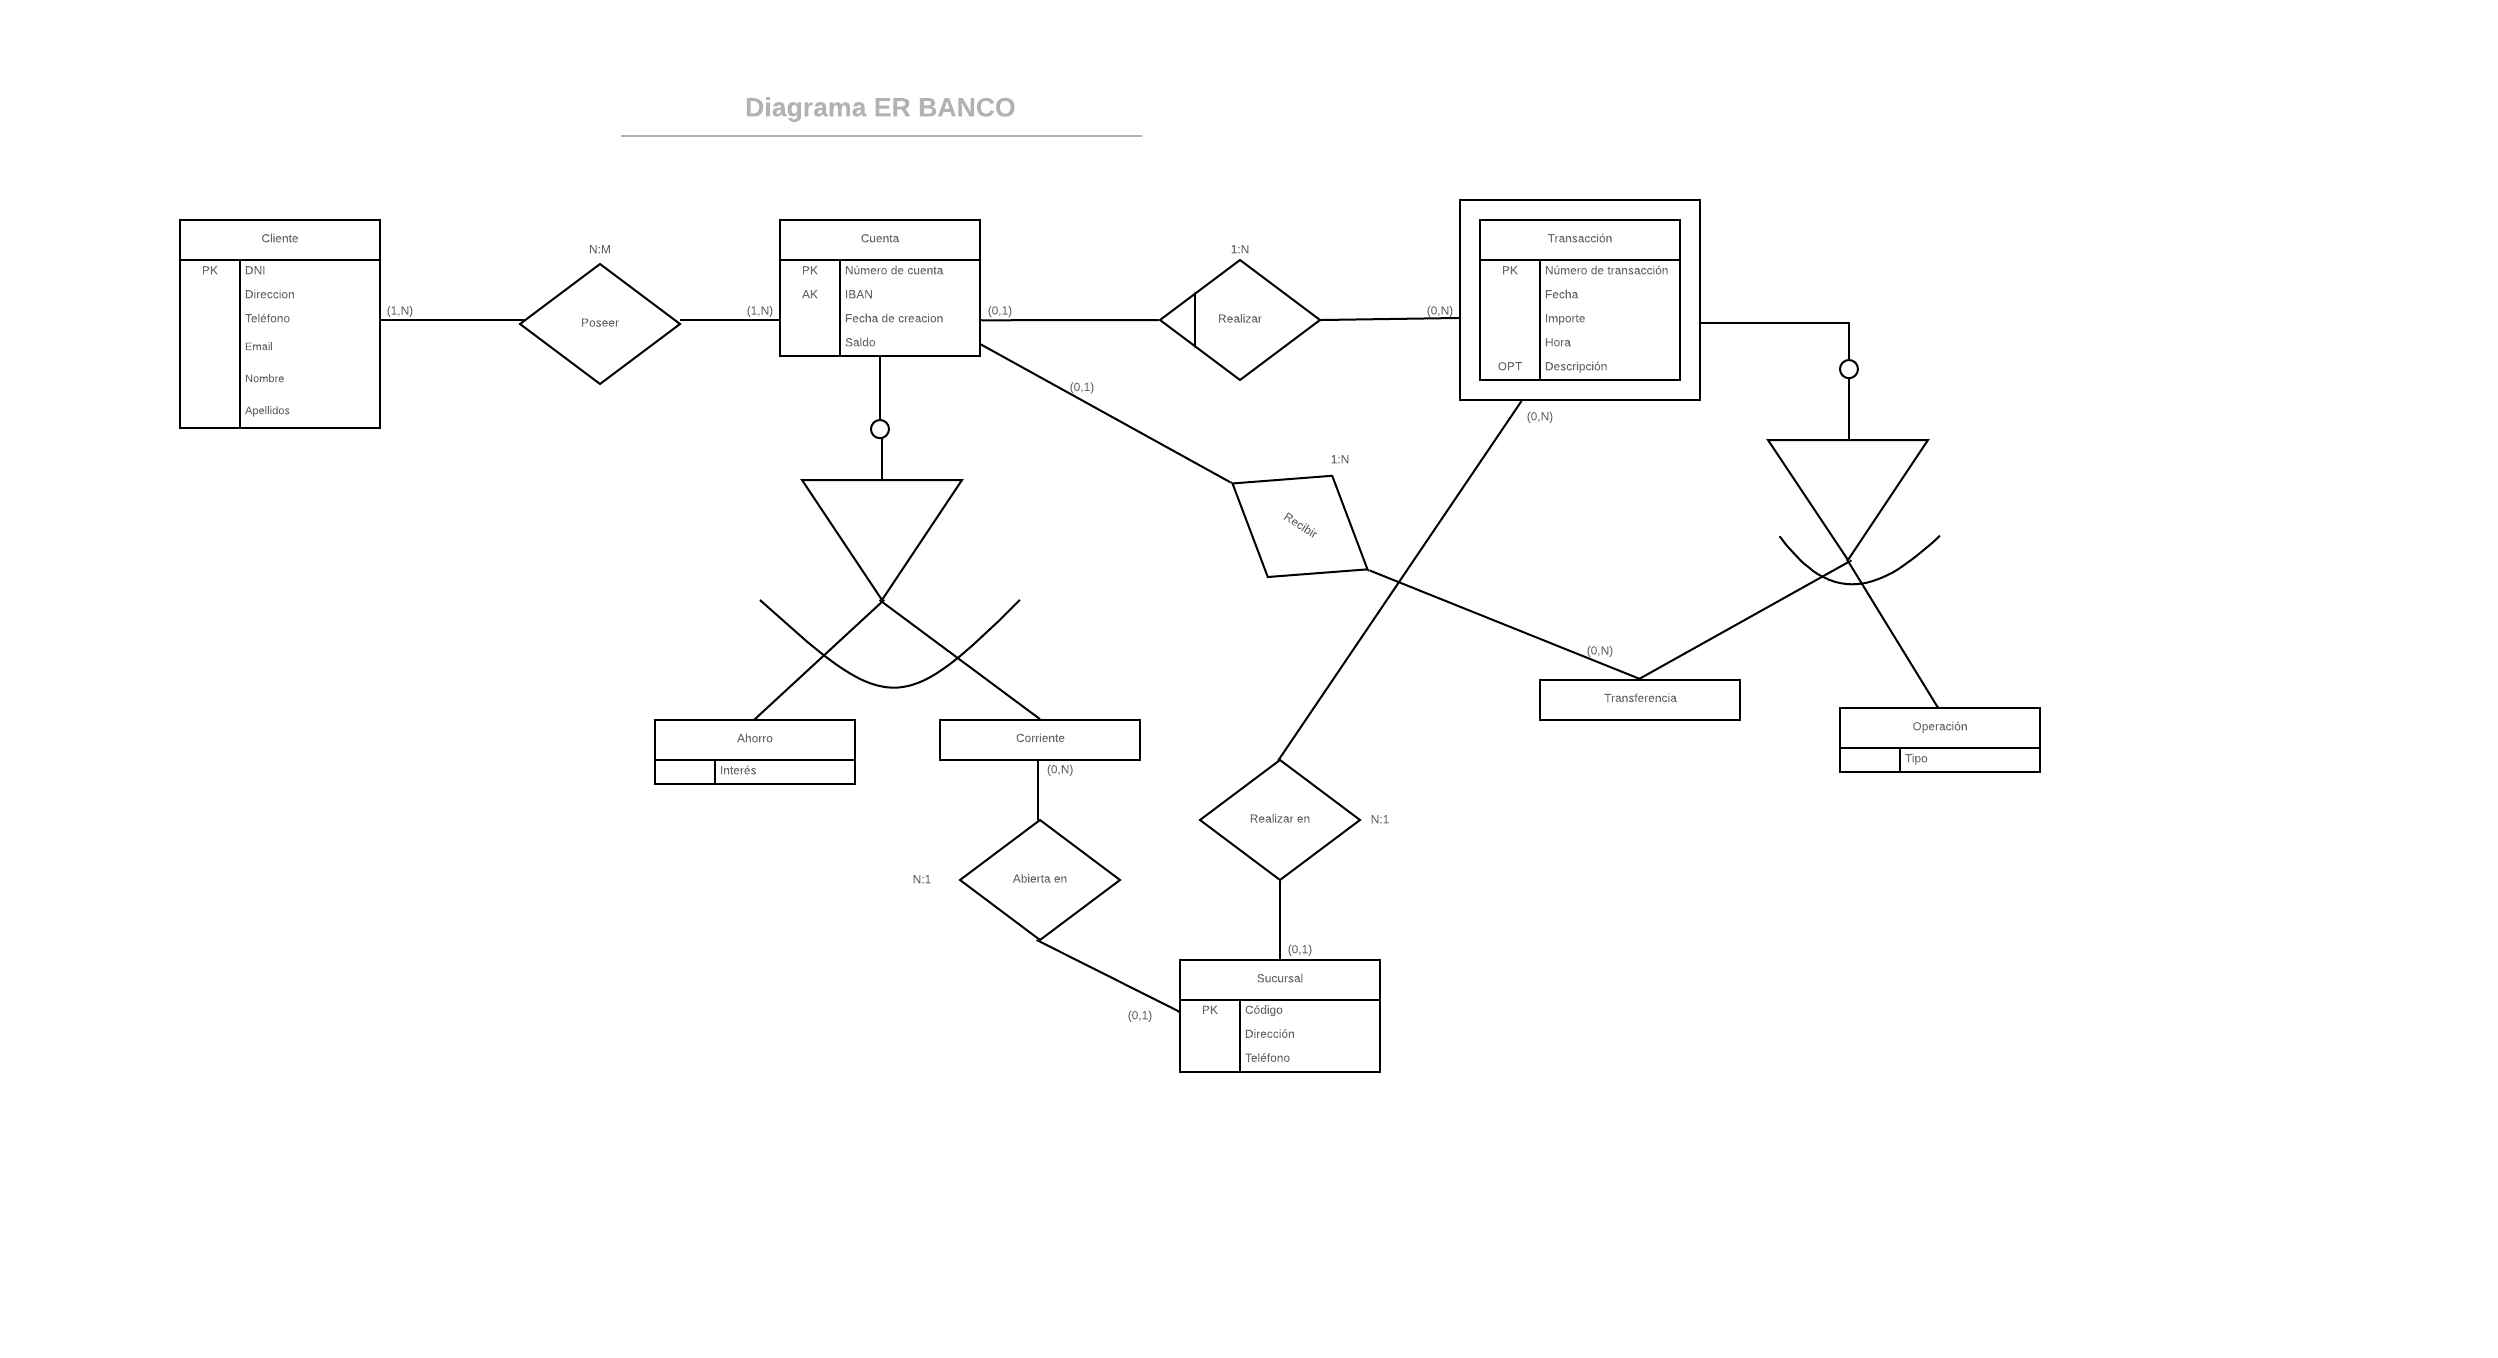
\includegraphics[scale=0.75]{images/diagramaer.png}
\caption{Diagrama ER de la Base de Datos bancaria de \emph{Banquito}}
\label{fig:diagramaer}
\end{figure}
\end{landscape}

\begin{figure}
\centering
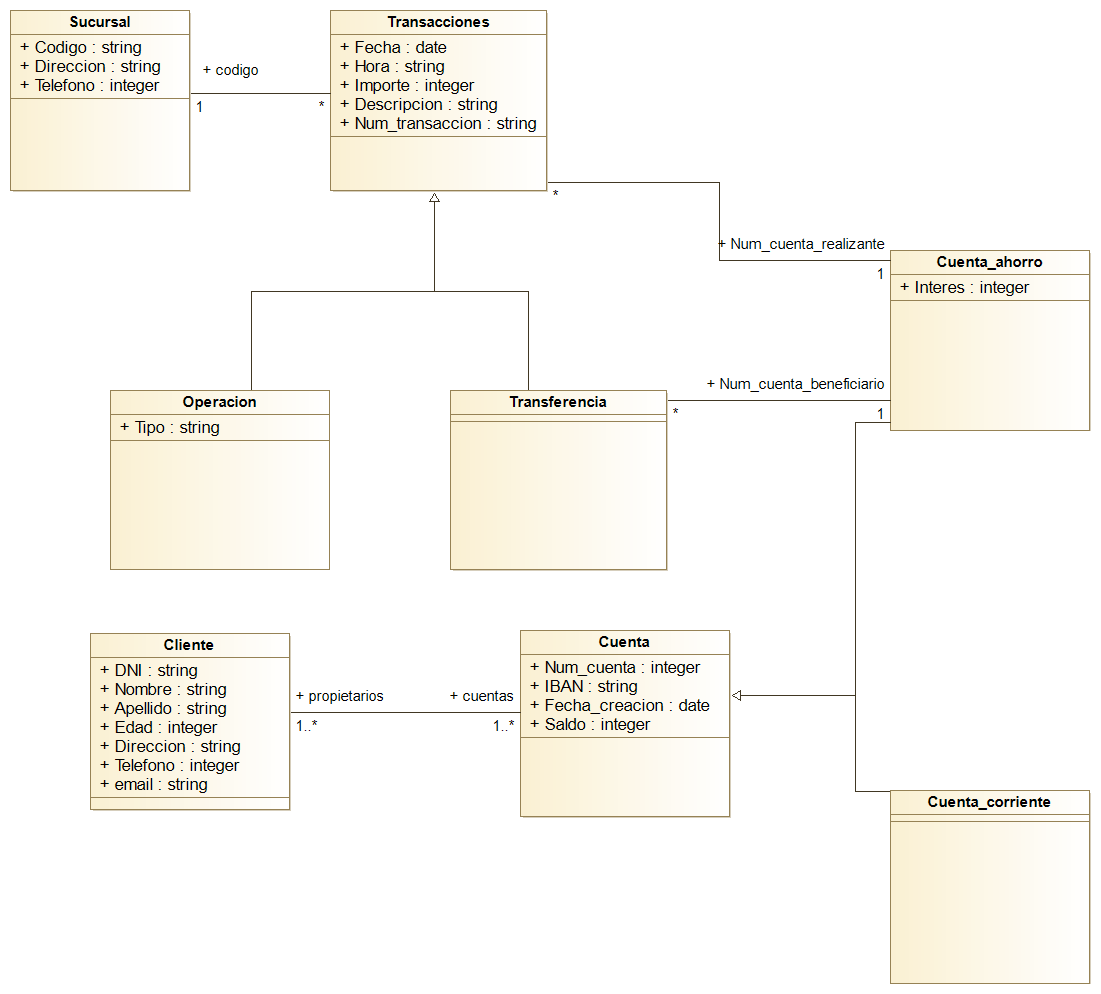
\includegraphics[scale=0.45]{images/diagramauml.png}
\caption{Diagrama de clases UML de la Base de Datos bancaria de \emph{Banquito}}
\label{fig:diagramauml}
\end{figure}

\begin{figure}
\centering
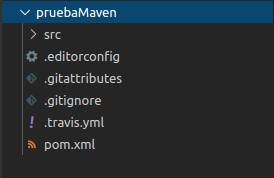
\includegraphics[scale=1]{images/estructuraMAVEN.png}
\caption{Estructura de un proyecto con la herramienta \emph{Apache Maven}}
\label{fig:estructuraMAVEN}
\end{figure}

\begin{landscape}
\begin{figure}
\centering
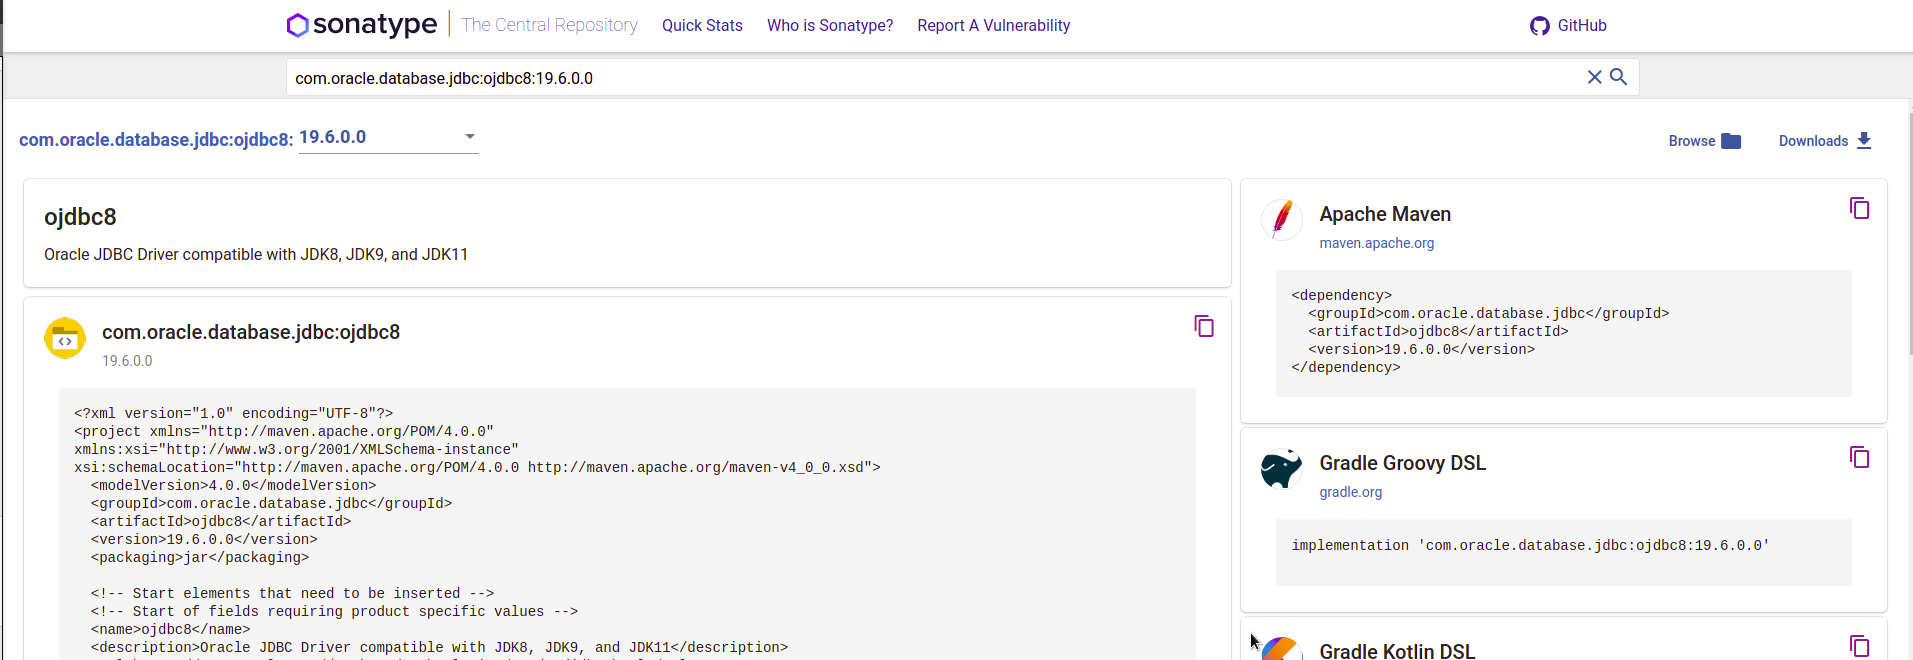
\includegraphics[scale=0.4]{images/mavenCentral.png}
\caption{Resultado de la búsqueda del Driver \emph{JDBC} de \emph{Oracle} en \emph{Maven Central}}
\label{fig:mavenCentral}
\end{figure}
\end{landscape}

\end{document}